\glsresetall
\chapter{Metodologia de Avaliação}
Neste capítulo, será apresentado como a solução foi avaliada. Particularmente, as perguntas que guiaram o desenvolvimento dos experimentos desenvolvidos para analisar a virtualização e a migração de processos no \nanvix foram:

\begin{enumerate}[label=(\roman*)]
    \item Qual o impacto do isolamento da \uarea e do código e dados de usuário sobre a execução do \nanvix?
    \item Qual a eficiência da migração de processos no \nanvix de acordo com a quantidade de estruturas manipuladas pela aplicação?
    \item Há sobrecarga no sistema de comunicação quando migramos apicações paralelamente?
\end{enumerate}

Para responder a primeira pergunta, foram desenvolvidos experimentos sobre a manipulação de \threads no \nanvix, que é o principal subsistema afetado pela \uarea. O experimento mensura os impactos na criação e junção de \threads através de diferentes perspectivas. Trata-se de um teste em que causamos um estresse no subsistema de \threads através da criação e junção do máximo de \threads que o sistema suporta. Especificamente, coletamos o tempo de execução, desvios e faltas ocorridas na \cache de dados e de instrução.

Para responder a segunda pergunta, foram desenvolvidos experimentos sobre a migração de processos no \nanvix. O experimento mensura o tempo de transferência de um processo entre \clusters de acordo com os recursos utilizados. Neste teste, variamos a quantidade de páginas de memória dinamicamente alocadas entre 0 e 32; e \threads usadas pela aplicação entre 1 e 17. Em resumo, neste experimento avaliamos como ocorre a progressão do tempo de transferência de um processo desde o mínimo de recursos utilizados (1 \thread e 0 páginas dinamicamente alocadas) até o máximo (17 \threads e 32 páginas dinamicamente alocadas).

Para responder a terceira pergunta, foi feito outro teste que mensura o \downtime da aplicação em diversos cenários. Neste teste, mensuramos o \downtime variando a quantidade de processos migrados paralelamente desde o mínimo (1 processo, envolvendo 2 \clusters) até o máximo (8 processos, envolvendo 16 \clusters).

Adicionalmente, um teste foi feito com o objetivo de garantir a capacidade do \daemon suportar múltiplas migrações. Neste experimento, um processo é migrado de \cluster em \cluster até que percorra todos os \clusters do processador \ie o processo é migrado realizando um movimento circular, passando do \cluster 0 para o 1, do 1 para o 2, e assim sucessivamente até retornar ao \cluster 0.

Todos os testes foram realizados no processador \mppa. Realizamos múltiplas replicações para garantir maior confiança estatística (100 replicações para o primeiro experimento e 20 replicações para o segundo e terceiro experimento). Para a medição de tempo no segundo e terceiro experimento, utilizamos a abstração de comunicação \sync. Em resumo, no início do teste todos os \clusters sincronizavam entre si através do \sync. Neste momento, o \iocluster iniciava uma contagem de ciclos. Ao final do experimento, todos os \clusters envolvidos sincronizavam novamente. Neste momento, o \iocluster parava a contagem de ciclos e esse era o tempo que a migração demorou até seu término. Destaca-se que nos experimentos que precisavam de algum \setup inicial, o tempo de \setup não foi considerado. Por exemplo, no segundo experimento, o tempo para a criação de \threads, alocação e manipulação das páginas dinamicamente alocadas não é contabilizado no tempo final. O resultado, portanto, engloba apenas o \downtime da aplicação.


\mytodo{citar o tamanho da aplicação. x paginas y threads, ...}

\chapter{Resultados Parciais}
\label{chap.results}

A solução foi avaliada em etapas anteriores ao desenvolvimento atual do trabalho e os resultados seguintes englobam apenas o susbsistema de \threads do \nanvix. 
% \todo{Seria bom colocar um capítulo de metodologia com perguntas que gostariamos de responder e detalhamento dos experimentos}
%
Para avaliar o impacto das mudanças feitas para a virtualização, foram desenvolvidos experimentos sobre a manipulação de \threads e suporte à migração de processos no \nanvix. Todos os experimentos foram executados no processador \mppa e os resultados mostrados são valores médios de 100 replicações de cada experimento para garantir 95\% de confiança estatística, resultando em um desvio padrão inferior a 1\%.

\begin{figure}[b]
	\centering
	\subcaptionminipage[fig.fork-join]%
                   {.5\textwidth}
                   {Tempo de criação de \threads.}
                   {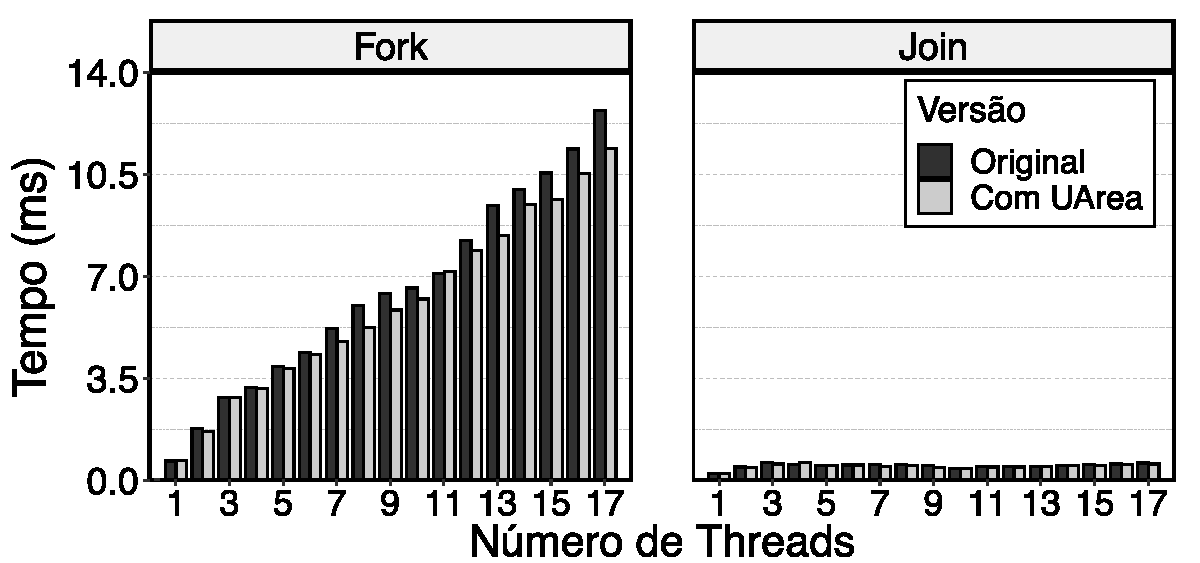
\includegraphics[width=\textwidth]{content/images/fork-join-kernel-time-bars.pdf}}
	\qquad
	\subcaptionminipage[fig.kernel-counters]
                   {.4\textwidth}
                   {Métricas do \kernel.}
                   {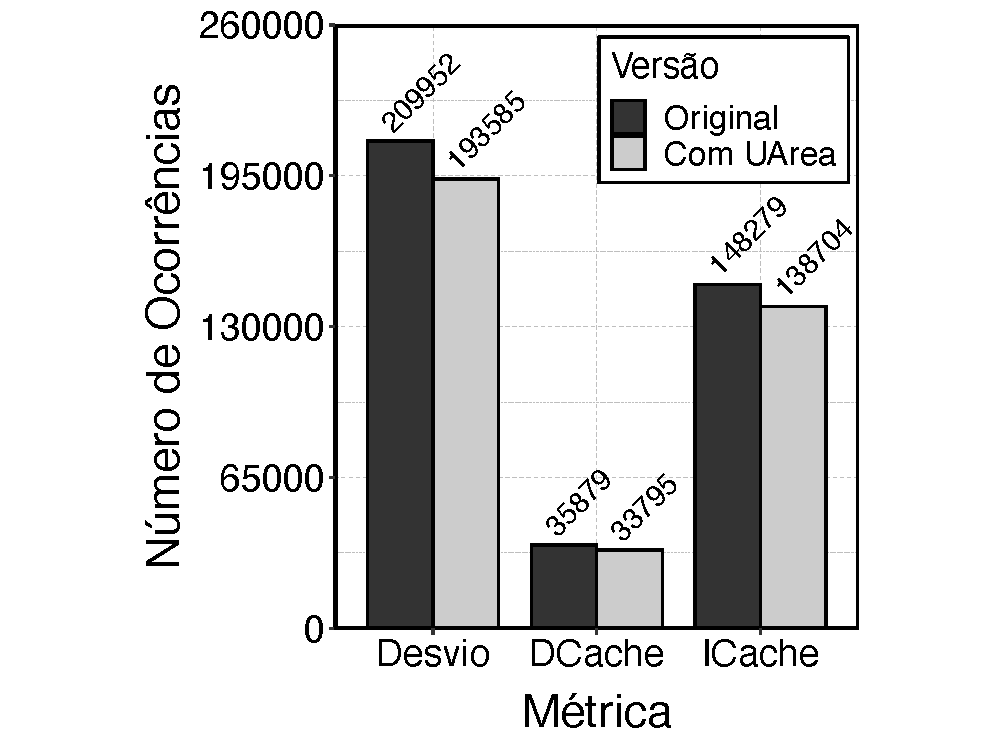
\includegraphics[width=\textwidth]{content/images/fork-join-kernel-counters.pdf}}
	\caption{Impactos da virtualização sobre a manipulação de \threads.\label{fig.threads}}%
\end{figure}

O experimento de manipulação de \threads mensura os impactos na criação e junção através de diferentes perspectivas. Especificamente, coletamos o tempo de execução, desvios e faltas ocorridas na \cache de dados e de instrução (\autoref{fig.threads}).
Os resultados apresentam um aumento no desempenho das operações de manipulação quando utilizamos a \uarea porque exploramos melhor a localidade espacial dos dados, o que, consequentemente, diminui o número de faltas na \cache.

O experimento de migração avaliou o tempo de transferência de um processo entre \clusters.
A aplicação de usuário migrada contém $352,8$~KB. Detalhadamente, foram transferidos instruções e dados ($342,8$~KB), a \uarea ($2$~KB) e uma pilha de execução ($8$~KB). O \downtime médio da aplicação, \ie o tempo que a aplicação demorou para restaurar a execução no \cluster destinatário após a migração, foi de $226$~ms. A média de tempo para o \cluster remetente enviar todos os dados foi de $218$~ms.